\documentclass[11pt,twocolumn]{article}
    \usepackage{fontspec} %connects to native fonts
    \usepackage{amsmath}
    \usepackage{mathtools}
    \usepackage{cleveref}
    \usepackage{pgfplots}
    \usepackage{graphicx}
    \usepackage{wrapfig}
    \usepackage{fancyref}
    \usepackage{amssymb}
    \usepackage{subfig}
    \usepackage{float}
    \usepackage[justification=RaggedRight, singlelinecheck=false, font={footnotesize}]{caption}
    \usepackage[portuguese]{babel}
    \usepackage[title,titletoc,toc]{appendix}
    \usepackage{fontspec}
    \usepackage[justification=centering]{caption}
    \begin{document}
    \pagenumbering{arabic}
    \bibliographystyle{plain}
    \title{
        \textnormal{
        \LARGE Universidade de Lisboa - Instituto Superior Técnico\\
        \Large Licenciatura em Engenharia Informática e de Computadores\\
        \Large Inteligência Artificial
    \\}
        \LARGE2º Projeto - Grupo 22
        \vspace{-1ex}
        }
    \author{Gonçalo Marques,
        \texttt{84719}
        \and
        Manuel Sousa,
        \texttt{84740}
    }
    \date{	\vspace{-1ex}
            \vspace{-4ex}
        }
    \maketitle
    
    \section*{P1}
    
    Começámos por elaborar um conjunto de features a aplicar sobre as palavras. De inicio contruímos features básicas que verificassem o numero de vogais e consoantes de uma palavra, o numero de acentos, etc. O primeiro objetivo passava apenas por estudar
    o comportamento do avaliador, e durante este processo, facilmente concluímos que quanto mais único fosse o output da feature em relação à palavra recebida, menor seria o erro.
    
    
    \begin{table}[htbp]
        \centering
        \caption{Analise individual dos erros de cada feature}
        \label{my-label}
        \begin{tabular}{|l|c|c|}
        \hline
        \multicolumn{1}{|c|}{Features Individuais}     & \textbf{Teste 1} & \textbf{Teste 2}                    \\ \hline
        [F1] N Acentos & 66.6 \%   & 23.1 \% \\ \hline
        [F2] N Vogais Par & 26.4 \%   & 23.1 \% \\ \hline
        [F3] N Vogais & 26.4 \%   & 34.8 \% \\ \hline
        [F4] N Consoantes   & 26.4 \%  & 23.1 \%      \\ \hline
        [F5] Palavras Repetidas   & 26.4 \%  & 23.1 \%      \\ \hline
        [F6] Palavra Par   & 23.1 \%  & 23.1 \%      \\ \hline
        [F7] Soma ASCII                             & 13.0 \%            & 12.2 \%                                \\ \hline
        [F8] Hash                             & 0.0 \%              & 0.0 \%                                \\ \hline
        \end{tabular}
        \end{table}
    \par

    Podemos observar que a função que soma o ASCII dos caracteres
    constituintes da palavra, tem um erro muito reduzido visto que o output dado pela feature será sempre único, menos quando palavras diferentes são constituídas pelos mesmos caracteres. 
    Assim, uma função que der um output único para cada palavra recebida iria dar um erro ainda mais baixo. Criámos uma função que gera um inteiro único para uma palavra (Hash), e desta maneira conseguimos obter uma percentagem de erro de 0\%.
    
    \begin{table}[htbp]
        \centering
        \caption{Analise coletiva dos erros com várias features}
        \label{my-label}
        \begin{tabular}{|l|c|c|}
        \hline
        \multicolumn{1}{|c|}{Features Coletivas}         & \textbf{Teste 1} & \textbf{Teste 2}                    \\ \hline
        [F5] + [F6] & 23.1 \% & 23.1 \% \\ \hline
        [F5] + [F6] + [F7]     & 7.7 \%  & 7.7 \%                   \\ \hline
        [F4] + [F5] + [F7] + [F8]   & 0.0 \%              & 0.0 \%                                 \\ \hline
        [F3] + [F4] + [F7]   & 6.4 \%             & 6.4 \%                                 \\ \hline
        [F3] + [F4] + [F7] + [F8]   & 0.0 \%          & 0.0 \%                                 \\ \hline
        \end{tabular}
        \end{table}
    \par  
    Por observação à tabela concluímos que a utilização de várias features produz um erro mais baixo, que usar features individuais. 
    Observamos também que a feature 8 é predominante, visto que a sua presença é suficiente para dar erro de 0\%. De forma a obter os melhores resultados (excluindo a feature 8), fomos ajustando as várias features até obter o melhor resultado possível. Para testar as features utilizámos 
    como classificador o K-Neighbours com 1 vizinho, porque teve um desempenho mais estável ao longo dos nossos testes.

\section*{P2}

Nesta secção usámos dois métodos de regressão não-linear: Epsilon-Support Vector Regression (SVR) e KernelRidge com kernel de Radial-basis function (KRR).
Usando validação cruzada (K-fold cross validation com um K=5), concluímos que as precisões de cada um destes métodos em ambos os testes são, respetivamente, (-0.17; -582.91) e (-0.10; -547.94).
A grande disparidade de precisão entre ambos os testes deve-se ao facto de os dados apresentados estarem dispostos exatamente de acordo com uma função de 3º grau no primeiro teste,
ao contrário do 2º teste, em que os valores estão muito mais dispersos.
Os parâmetros foram ajustados de maneira a modelarem mais precisa e corretamente os dados apresentados em ambas as situações.
Concluímos então que o método KRR tem melhor precisão no caso apresentado.

\section*{P3}

As imagens seguintes ilustram a maneira como o agente se movimenta pelos ambientes 1 e 2, incluíndo uma representação gráfica dos mesmos:
	
\begin{figure}[htbp]
    \begin{center}
        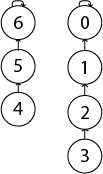
\includegraphics[scale=0.3]{Trajetoria1.png}
        \caption[justification=centering]{Percurso do agente no ambiente 1}
    \end{center}
    \end{figure}
    
    \begin{figure}[htbp]
    \begin{center}
        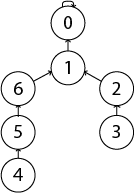
\includegraphics[scale=0.3]{Trajetoria2.png}
        \caption{Percurso do agente no ambiente 2}
    \end{center}
    \end{figure}
    
    Na trajetória 1, existem dois estados-objetivos , o estado 6 e o estado 0. Se o agente começar no estado 4, 5 ou 6, vai-se dirigir
    sempre em direção do estado 6, visto que é o estado-objetivo mais próximo. Caso contrário vai-se dirigir em direção ao estado 0.
    
    Na trajetória 2, existe apenas um estado-objetivo 0. Nesta situação, o agente vai-se dirigir sempre em direção ao estado 1,
    sendo a única maneira de chegar ao estado-objetivo, que apenas se consegue aceder através do estado 1.
    
    A função de recompensa, f(x) = y, em que x corresponde ao estado em que o agente se encontra e y é a recompensa de executar uma ação nesse estado,
    é a seguinte para ambas as trajetórias\par
    
    \begin{figure}[htbp]
    \begin{center}
        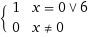
\includegraphics[scale=0.6]{piece1.png}
        \caption{Função Recompensa}
    \end{center}
    \end{figure}


\end{document}
